%%%%%%%%%%%%%%
%% Run LaTeX on this file several times to get Table of Contents,
%% cross-references, and citations.

%% If you have font problems, you may edit the w-bookps.sty file
%% to customize the font names to match those on your system.

%% w-bksamp.tex. Current Version: Feb 16, 2012
%%%%%%%%%%%%%%%%%%%%%%%%%%%%%%%%%%%%%%%%%%%%%%%%%%%%%%%%%%%%%%%%
%
%  Sample file for
%  Wiley Book Style, Design No.: SD 001B, 7x10
%  Wiley Book Style, Design No.: SD 004B, 6x9
%
%
%  Prepared by Amy Hendrickson, TeXnology Inc.
%  http://www.texnology.com
%%%%%%%%%%%%%%%%%%%%%%%%%%%%%%%%%%%%%%%%%%%%%%%%%%%%%%%%%%%%%%%%

%%%%%%%%%%%%%
% 7x10
%\documentclass{wileySev}

% 6x9
\documentclass{wileySix}

\usepackage{graphicx}
\usepackage{listings}

\usepackage{color}
 
\definecolor{codegreen}{rgb}{0,0.6,0}
\definecolor{codegray}{rgb}{0.5,0.5,0.5}
\definecolor{codepurple}{rgb}{0.58,0,0.82}
\definecolor{backcolour}{rgb}{0.95,0.95,0.92}
 
\lstdefinestyle{mystyle}{
    backgroundcolor=\color{backcolour},   
    commentstyle=\color{codegreen},
    keywordstyle=\color{magenta},
    numberstyle=\tiny\color{codegray},
    stringstyle=\color{codepurple},
    basicstyle=\footnotesize,
    breakatwhitespace=false,         
    breaklines=true,                 
    captionpos=b,                    
    keepspaces=true,                 
    numbers=left,                    
    numbersep=5pt,                  
    showspaces=false,                
    showstringspaces=false,
    showtabs=false,                  
    tabsize=2,
    language=sh
}
 
\lstset{style=mystyle}

%%%%%%%
%% for times math: However, this package disables bold math (!)
%% \mathbf{x} will still work, but you will not have bold math
%% in section heads or chapter titles. If you don't use math
%% in those environments, mathptmx might be a good choice.

% \usepackage{mathptmx}

% For PostScript text
\usepackage{w-bookps}

%%%%%%%%%%%%%%%%%%%%%%%%%%%%%%%%%%%%%%%%%%%%%%%%%%%%%%%%%%%%%%%%
%% Other packages you might want to use:

% for chapter bibliography made with BibTeX
% \usepackage{chapterbib}

% for multiple indices
% \usepackage{multind}

% for answers to problems
% \usepackage{answers}

%%%%%%%%%%%%%%%%%%%%%%%%%%%%%%
%% Change options here if you want:
%%
%% How many levels of section head would you like numbered?
%% 0= no section numbers, 1= section, 2= subsection, 3= subsubsection
%%==>>
\setcounter{secnumdepth}{3}

%% How many levels of section head would you like to appear in the
%% Table of Contents?
%% 0= chapter titles, 1= section titles, 2= subsection titles, 
%% 3= subsubsection titles.
%%==>>
\setcounter{tocdepth}{2}

%% Cropmarks? good for final page makeup
%% \docropmarks

%%%%%%%%%%%%%%%%%%%%%%%%%%%%%%
%
% DRAFT
%
% Uncomment to get double spacing between lines, current date and time
% printed at bottom of page.
% \draft
% (If you want to keep tables from becoming double spaced also uncomment
% this):
% \renewcommand{\arraystretch}{0.6}
%%%%%%%%%%%%%%%%%%%%%%%%%%%%%%

%%%%%%% Demo of section head containing sample macro:
%% To get a macro to expand correctly in a section head, with upper and
%% lower case math, put the definition and set the box 
%% before \begin{document}, so that when it appears in the 
%% table of contents it will also work:

\newcommand{\VT}[1]{\ensuremath{{V_{T#1}}}}

%% use a box to expand the macro before we put it into the section head:

\newbox\sectsavebox
\setbox\sectsavebox=\hbox{\boldmath\VT{xyz}}

%%%%%%%%%%%%%%%%% End Demo


\begin{document}


\booktitle{Cerdas Menguasai Python}
\subtitle{Dalam 24 Jam}

\authors{Rolly M. Awangga\\
\affil{Informatics Research Center}
%Floyd J. Fowler, Jr.\\
%\affil{University of New Mexico}
}

\offprintinfo{Cerdas Menguasai Python, First Edition}{Rolly M. Awangga}

%% Can use \\ if title, and edition are too wide, ie,
%% \offprintinfo{Survey Methodology,\\ Second Edition}{Robert M. Groves}

%%%%%%%%%%%%%%%%%%%%%%%%%%%%%%
%% 
\halftitlepage

\titlepage


\begin{copyrightpage}{2019}
\input{info/copyrightpage}
\end{copyrightpage}

\dedication{`Jika Kamu tidak dapat menahan lelahnya belajar, 
Maka kamu harus sanggup menahan perihnya Kebodohan.'
~Imam Syafi'i~}

\begin{contributors}
\input{info/contributors}
\end{contributors}

\contentsinbrief
\tableofcontents
\listoffigures
\listoftables
\lstlistoflistings


\begin{foreword}
\input{info/foreword}
\end{foreword}

\begin{preface}
\input{info/preface}
\end{preface}


\begin{acknowledgments}
\input{info/acknowledgments}
\end{acknowledgments}

\begin{acronyms}
\input{info/acronyms}
\end{acronyms}

\begin{glossary}
\input{info/glossary}
\end{glossary}

\begin{symbols}
\input{info/symbols}
\end{symbols}

\begin{introduction}
\input{info/introduction}
\end{introduction}

%%%%%%%%%%%%%%%%%%Isi Buku_
\chapter{Sejarah Python}
Python dikembangkan oleh Guido van Rossum pada tahun 1990-an di CWI, Amsterdam sebagai kelanjutan
dari bahasa pemrograman ABC. Versi terakhir yang dikeluarkan CWI adalah 1.2. Tahun 1995, Guido pindah
ke CNRI sambil terus melanjutkan pengembangan Python. Versi terakhir yang dikeluarkan adalah 1.6. Tahun
2000, Guido dan para pengembang inti Python pindah ke BeOpen.com yang merupakan sebuah perusahaan
komersial dan membentuk BeOpen PythonLabs. Python 2.0 dikeluarkan oleh BeOpen. Setelah
mengeluarkan Python 2.0, Guido dan beberapa anggota tim PythonLabs pindah ke DigitalCreations. Saat ini
pengembangan Python terus dilakukan oleh sekumpulan pemrogram yang dikoordinir Guido dan Python
Software Foundation. Python Software Foundation adalah sebuah organisasi non-profit yang dibentuk
sebagai pemegang hak cipta intelektual Python sejak versi 2.1 dan dengan demikian mencegah Python
dimiliki oleh perusahaan komersial. Saat ini distribusi Python sudah mencapai versi 2.7.13 dan versi 3.6.0.

Nama Python dipilih oleh Guido sebagai nama bahasa ciptaannya karena kecintaan guido pada acara televisi
Monty Python’s Flying Circus. Oleh karena itu seringkali ungkapan-ungkapan khas dari acara tersebut
seringkali muncul dalam korespondensi antar pengguna Python.

\chapter{Perbedaan Python 2 Dan paython 3}
Python 2
Dipublikasikan pada akhir tahun 2000, Python 2 dinilai lebih transparan dan inklusif untuk pengembangan software ketimbang versi sebelumnya. Hal ini didukung dengan adanya PEP – Python Enhancement Proposal, sebuah spesifikasi teknis yang menjadi tuntunan informasi untuk penggunanya dan menggambarkan fitur baru pada Python itu sendiri.

Sebagai tambahan, Python 2 dilengkapi dengan berbagai fitur programatikal seperti cycle-detecting garbage collector untuk mengotomasi manajemen memori, peningkatan dukungan untuk Unicode, list comprehension untuk membuat sebuah list berdasarkan list yang sudah ada. Unifikasi pada tipe data Python dan class ke satu hirarki terjadi pada rilis Python 2.2

Python 3
Python 3 diharapkan sebagai masa depan Python dan merupakan versi yang saat tulisan ini dibuat masih aktif dikembangkan. Python 3 sendiri adalah versi dengan banyak perubahan yang dirilis akhir tahun 2008. Fokus dari Python 3 itu sendiri adalah untuk melakukan perapian pada codebase dan menghapuskan duplikasi (redundancy). Perubahan terbesar pada Python 3 termasuk memasukkan statemen print ke dalam built-in function.

Awalnya, Python 3 mengalami hambatan pada pengadopsiannya. Itu akibat dari tidak adanya backwards compatibility dengan Python 2. Hal ini membuat pengguna Python sangat berat hati untuk pindah ke versi 3 ini. Tambahannya, banyak sekali library yang hanya tersedia untuk Python 2., tapi setelah tim pengembangan di balik Python 3 telah berulang kali menjelaskan bahwa dukungan terhadap Python 2 akan segera dihentikan, dan semakin banyak libary disalin ke Python 3, maka penerapan Python 3 semakin lama semakin meningkat.


\chapter{Cara Instalasi Python}

Dalam Menginstal Python terlebih dahulu download python di web resmi. dalam cara instalisasi python sebagai contoh menggunakan python 3.7
\begin{figure}[!htbp]
\centering
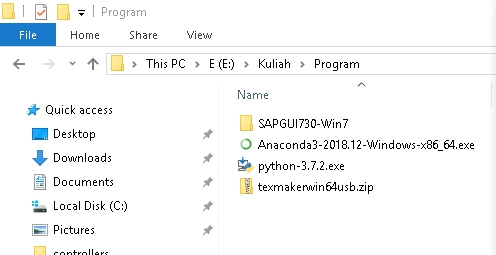
\includegraphics[width=3cm,height=3cm]{1.jpg}
\caption{1.jpg}
\label{penanda}
\end{figure}


Setelah Proses tersebut kita akan memulai proses berikutya, dalam proses ini akan menjelaskan tentang proses penginstalan ,Centang Install launcher for all user untuk mengaktifkan python pada semua user 
Windows dan centang Python 3.7 to PATH untuk menambah path command Python. Kemudian klik Install Now. Klik Yes saat muncul notifikasi User Account Control.
\begin{figure}[!htbp]
\centering
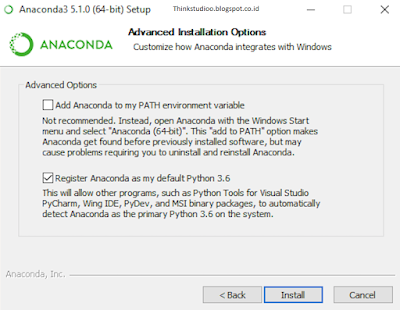
\includegraphics[width=3cm,height=3cm]{2.png}
\caption{2.png}
\label{penanda}
\end{figure}

setelah proses tersebut maka proses instalasi yang akan memakan waktu yang cukup lama.
\begin{figure}[!htbp]
\centering
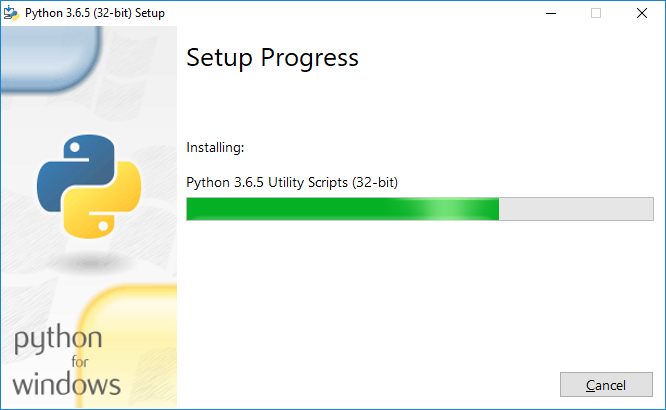
\includegraphics[width=3cm,height=3cm]{3.png}
\caption{3.png}
\label{penanda}
\end{figure}
\bibliographystyle{IEEEtran} 
%\def\bibfont{\normalsize}
\bibliography{references}

Setelah Proses instalasi berhasil maka Akan muncul Gambar seperti dibawah ini.
\begin{figure}[!htbp]
\centering
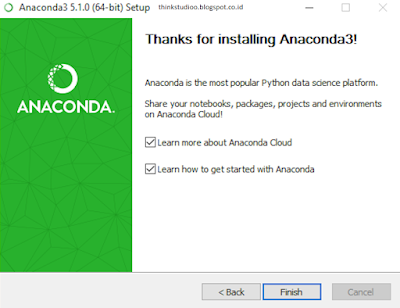
\includegraphics[width=3cm,height=3cm]{4.png}
\caption{4.png}
\label{penanda}
\end{figure}

\chapter{Cara Instalasi Anaconda}
Dalam Proses Instalasi Setelah didownload, klik  kali pada installer Anaconda. Kemudian klik next.
\begin{figure}[!htbp]
\centering
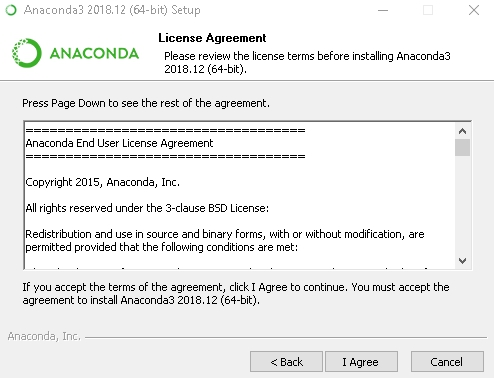
\includegraphics[width=3cm,height=3cm]{12.jpg}
\caption{4.jpg}
\label{penanda}
\end{figure}


\bibliographystyle{IEEEtran} 
%\def\bibfont{\normalsize}
w\bibliography{references}


%%%%%%%%%%%%%%%
%%  The default LaTeX Index
%%  Don't need to add any commands before \begin{document}
\printindex

%%%% Making an index
%% 
%% 1. Make index entries, don't leave any spaces so that they
%% will be sorted correctly.
%% 
%% \index{term}
%% \index{term!subterm}
%% \index{term!subterm!subsubterm}
%% 
%% 2. Run LaTeX several times to produce <filename>.idx
%% 
%% 3. On command line, type  makeindx <filename> which
%% will produce <filename>.ind 
%% 
%% 4. Type \printindex to make the index appear in your book.
%% 
%% 5. If you would like to edit <filename>.ind 
%% you may do so. See docs.pdf for more information.
%% 
%%%%%%%%%%%%%%%%%%%%%%%%%%%%%%

%%%%%%%%%%%%%% Making Multiple Indices %%%%%%%%%%%%%%%%
%% 1. 
%% \usepackage{multind}
%% \makeindex{book}
%% \makeindex{authors}
%% \begin{document}
%% 
%% 2.
%% % add index terms to your book, ie,
%% \index{book}{A term to go to the topic index}
%% \index{authors}{Put this author in the author index}
%% 
%% \index{book}{Cows}
%% \index{book}{Cows!Jersey}
%% \index{book}{Cows!Jersey!Brown}
%% 
%% \index{author}{Douglas Adams}
%% \index{author}{Boethius}
%% \index{author}{Mark Twain}
%% 
%% 3. On command line type 
%% makeindex topic 
%% makeindex authors
%% 
%% 4.
%% this is a Wiley command to make the indices print:
%% \multiprintindex{book}{Topic index}
%% \multiprintindex{authors}{Author index}

\end{document}

